\documentclass{report}
\usepackage{graphicx} % Required for inserting images
\usepackage[italian]{babel}
\usepackage{tikz}
\usepackage{hyperref}
\usepackage{amsmath}
\usepackage{xcolor}

\definecolor{darkgreen}{rgb}{0.0, 0.5, 0.0}


\title{Sistemi Biometrici basati sull'Iride}
\date{Parte V}

\begin{document}

\maketitle

\tableofcontents
\newpage


\chapter{Caratteristiche dell'iride e creazione dell'Iriscode}

L'iride è considerato il tratto biometrico più accurato
dopo il DNA. È poco gradito dagli utenti per la sua
"percepita" invasività.

\noindent L'iride presenta caratteristiche numerosissime e stabili 
nel tempo; inizia a crearsi dal terzo mese nel feto, al settimo mese 
il processo è completato ma diventa stabile dal secondo anno di vita.

\noindent Il sistema è piuttosto complesso e costoso, ma difficile da frodare.

\section{Vantaggi e svantaggi}

Tra i \textbf{\textcolor{green}{vantaggi}} troviamo:
\begin{itemize}
    \item acquisizione senza contatto
    \item molte caratteristiche casuali e distintive
    \item il tratto appartiene ad un organo interno generalmente protetto e presente in tutta la popolazione
    \item esistono sistemi di acquisizione ed elaborazione molto veloci
\end{itemize}
Tra gli \textbf{\textcolor{red}{svantaggi}} troviamo:
\begin{itemize}
    \item l'acquisizione può essere difficile 
    \item l'iride è piatta ma è dietro una superficie curva e bagnata (cornea)
    \item una buona parte è nascosta da ciglia e palpebra
    \item si deforma con la dilatazione della pupilla
    \item invecchiando possono comparire delle pigmentazioni non presenti
    precedentemente
\end{itemize}

\section{Struttura dell'iride}
L'iride è una \textbf{membrana piatta che sta tra la cornea e il cristallino.}
Ha il compito di controllare il livello di intensità luminosa che deve entrare nell'occhio.

La \textbf{cornea} è una struttura trasparente a forma di cupola 
posizionata nella parte anteriore al centro della sclera (parte bianca).

Il \textbf{cristallino} è una lente elastica, trasparente, le cui contrazioni muscolari ne 
permettono l'ispessimento o restringimento per consentire all'occhio di mettere a fuoco oggetti 
posti a distanze diverse.

\begin{figure}[ht]
    \centering
    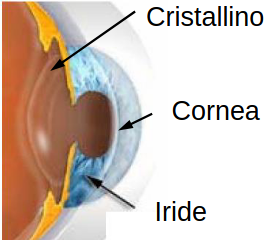
\includegraphics[width=0.4\linewidth]{images/struttura-iride.png}
\end{figure}

\section{Unicità dell'iride}

Come nel caso delle impronte, \textbf{non esistono due iridi uguali}.

\noindent Durante la formazione dell'iride si hanno delle componenti casuali che 
producono un pattern di righe, tagli e pieghe (le feature iridee) \textbf{unico
e distinguibile}.

\noindent Anche i gemelli omozigoti hanno iridi diverse.

\begin{figure}[ht]
    \centering
    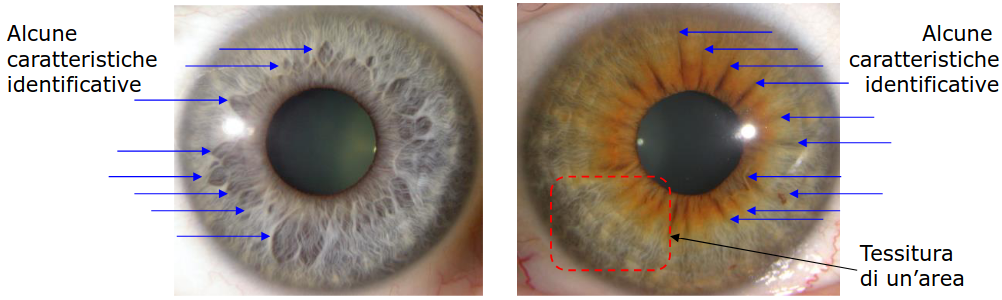
\includegraphics[width=1\linewidth]{images/unicita.png}
\end{figure}

\noindent Le feature più interessanti per il sistema biometrico si \textbf{vedono meglio con luce IR} 
piuttosto che la luce visibile.

\noindent È necessario inoltre usare \textbf{telecamere con ottiche variabili} per trovare
l'occhio nel volto e poi zoomare verso l'occhio per acquisirlo alla massima
risoluzione possibile.

\section{Rappresentazione delle iridi}
I moderni sistemi per il riconoscimento basati sull'iride rappresentano l'iride come 
una stringa di bit, chiamata \textbf{iriscode}.

\noindent I passi che permettono di passare da una immagine di un occhio ad un iriscode sono:
\begin{enumerate}
    \item individuazione dei centri e raggi della pupilla e dell'iride 
    \item rimozione della parte non utile occupata da ciglia 
    \item linearizzazione dell'iride
    \item trasformazione dell'iride linearizzata in wavelet
    \item trasformazione della trasformata wavelet in bit, ovvero iriscode
\end{enumerate}

\subsection{Calcolo dei centri e raggi di iride e pupilla}
Viene trovato l'occhio nell'immagine del volto, successivamente la pupilla 
e il raggio esterno dell'iride.

\subsection{Rimozione di palpebre e ciglia}
Solo una parte dell'iride è utile al riconoscimento; occorre segmentare 
solo la parte utile dell'iride.

\noindent Se manca più del 50\% dell'iride occorre riacquisire l'immagine.

\subsection{Linearizzaione dell'iride}
Per aumentare l'efficienza degli algoritmi, l'iride non viene elaborata
direttamente nell'immagine in ingresso ma convertita in un rettangolo.

\noindent Questa operazione viene fatta passando da delle coordinate cartesiane $(x, y)$ a polari $(r, 0)$.
\begin{figure}[ht]
    \centering
    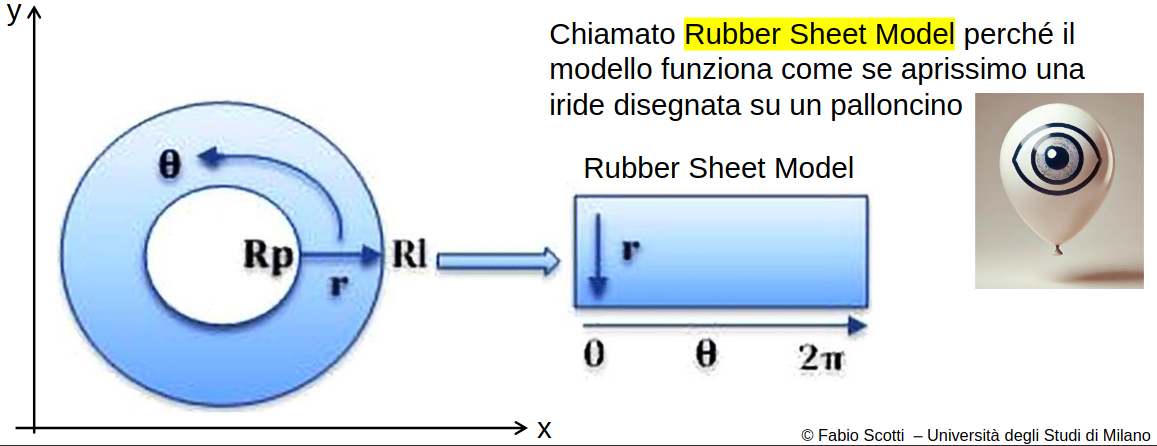
\includegraphics[width=1\linewidth]{images/linear-1.png}
\end{figure}

\begin{enumerate}
    \item vengono individuati i raggi e centri
    \item si fissano le dimensioni dei settori dell'iride, 
    scegliendo numero di corone e ampiezza dell'angolo di scansione
    \item ogni pixel del \textit{rubber sheet model} è la media del colore del relativo settore
\end{enumerate}


\begin{figure}[ht]
    \centering
    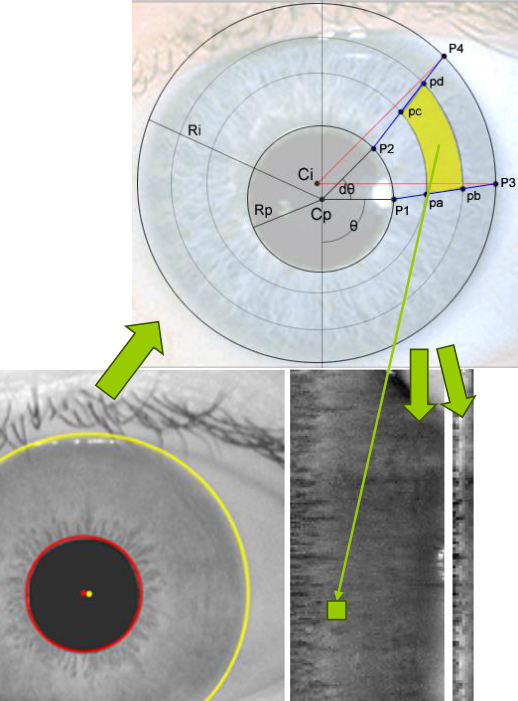
\includegraphics[width=0.5\linewidth]{images/linear-2.png}
\end{figure}

\newpage
\section{Proprietà dell'iris code}

\begin{itemize}
    \item La codifica dell'iride avviene in uno spazio 2D, rendendo la codifica \textbf{invariante}
    rispetto a:
    \begin{itemize}
        \item dimensione dell'iride
        \item zoom dei sistemi ottici
        \item e dilatazione dell'iride
    \end{itemize}
    \item È \textbf{invariante} rispetto a:
    \begin{itemize}
        \item contrasto dell'immagine 
        \item livello di grigio medio nell'immagine 
        \item illuminazione
    \end{itemize}
    \item È \textbf{molto compatto}, di solito bastano 256 byte per rappresentare una iride, più altri 
    256 byte di controllo per escludere i bit dovuti ad artefatti (\textit{riflessi sulla cornea, ciglia, palpebre, troppo poco contrasto})
    \item La probabilità di ogni bit di essere 1 è pari al 50\%
    
    $\rightarrow$ l'iriscode è un codice a \textbf{massima entropia}
\end{itemize}

\chapter{Algoritmi di enhancement e prefiltraggio}

\section{Controllo qualità del sample}
\begin{figure}[ht]
    \centering
    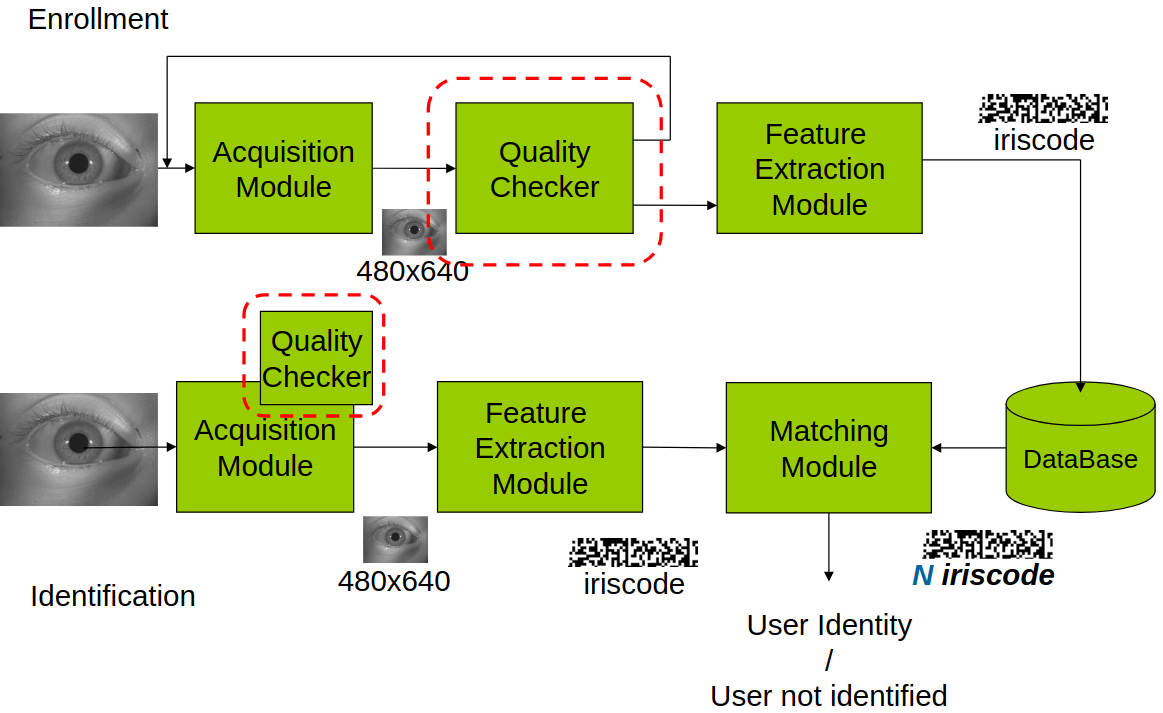
\includegraphics[width=1\linewidth]{images/prefiltraggio.png}
\end{figure}


\subsection{Focus assessement}
La probabilità di avere una iride già a fuoco è molto bassa, perché:
\begin{itemize}
    \item ingrandimento del sistema ottico 
    \item l'occhio si muove rapidamente (micromovimenti non controllabili)
    \item illuminazione limitata
\end{itemize}

\noindent Per questo il fuoco dell'iride viene controllato con dei filtri
software.\\


\noindent L'effetto di sfocatura dovuto ad un sistema ottico può essere parzialmente riconvertito
usando un \textbf{filtro di deblur}, che si comporta al "contrario" della parte 
che produce la sfocatura:
\begin{itemize}
    \item tende ad aumentare le frequenze alte dell'immagine che erano state attenuate dal blur 
    \item può essere seguito a livello di frame (le prestazioni lo consentono)
\end{itemize}

\subsection{Acquisizioni fuori fuoco}
Se l'immagine è troppo mossa occorre scartarla, in quanto l'iriscode risultante 
sarebbe composto solo da bit casuali dipendenti dal rumore 

$\rightarrow$ se fosse eseguito un enroll con un template simile si avrebbe sicuramente un false non-match

\noindent Il controllo equivale a verificare se è presente una sufficiente quantità di
"dettagli fini" maggiore di una determinata soglia.

\section{Contrast Adjustment}
Non si usano particolari algoritmi di prefiltraggio nel caso dell'iride;
in alcuni casi si applica un \textbf{constrast stretching} per migliorare il contrasto 
e quindi la leggibilità dell'immagine.

\newpage
\section{Modulo Estrazione delle Feature}

\begin{figure}[ht]
    \centering
    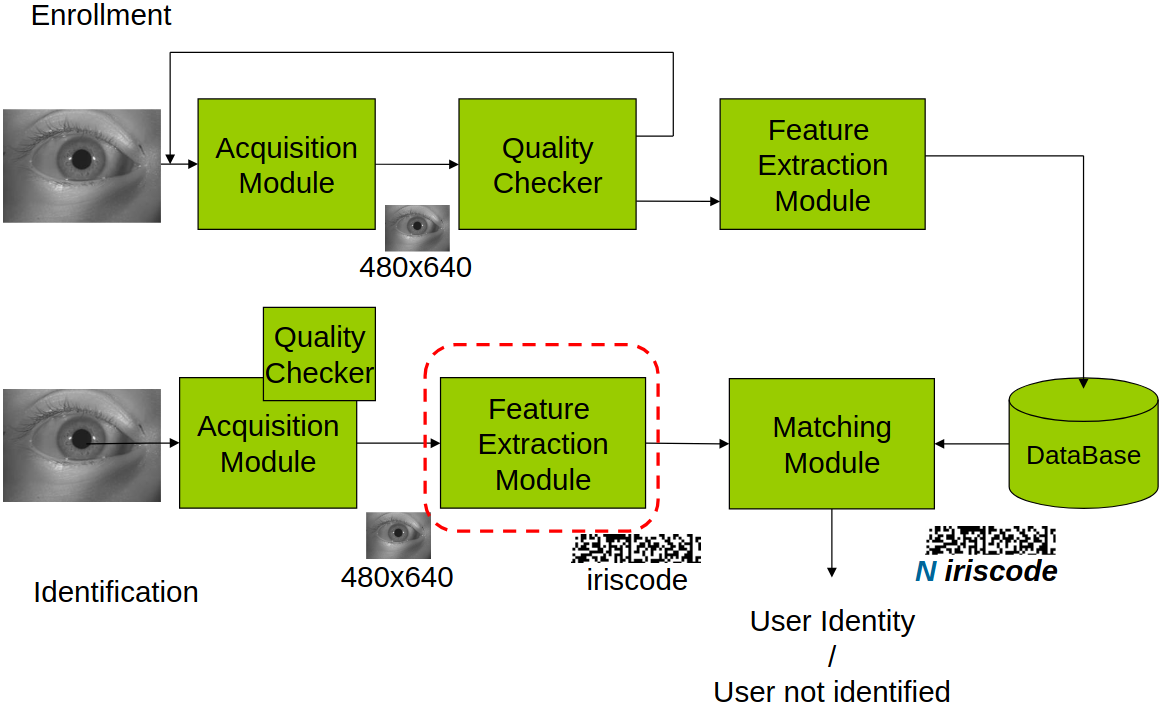
\includegraphics[width=1\linewidth]{images/estrazione-features.png}
\end{figure}

\subsection{Come trovare l'iride}
Si cercano nell'immagine i centri di contorni di variazioni di grigio di forma circolare.

\begin{figure}[ht]
    \centering
    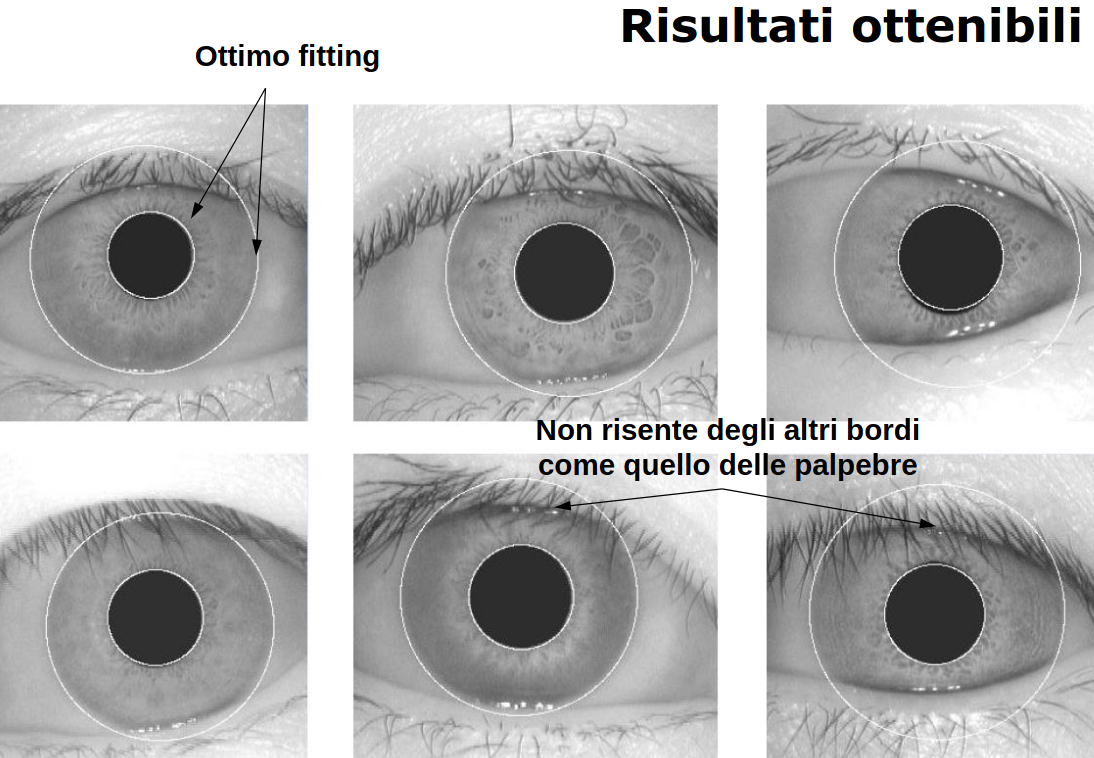
\includegraphics[width=0.6\linewidth]{images/ricerca-iride.png}
\end{figure}

\subsubsection{Estrazione delle palpebre}
\noindent Modificando gli operatori della formula è possibile trovare le palpebre, 
immaginandole come parte di una parabola.

\begin{figure}[ht]
    \centering
    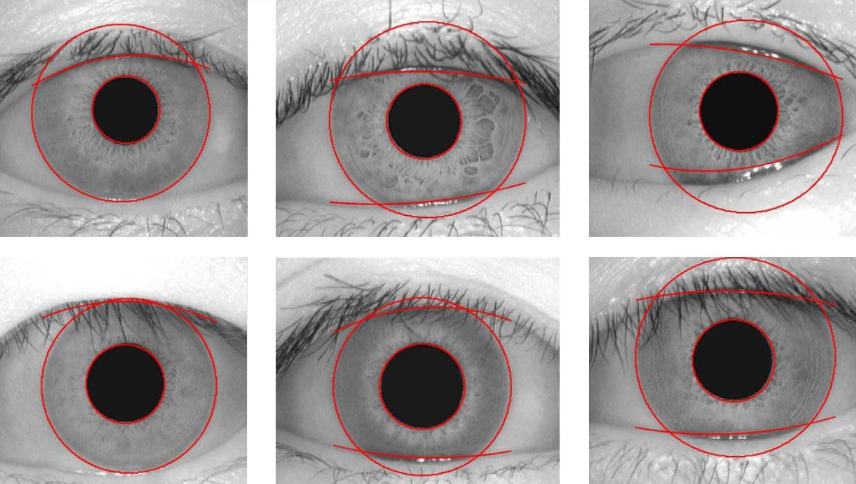
\includegraphics[width=0.5\linewidth]{images/estrazione-palpebre.png}
\end{figure}



\subsubsection{Estrazione delle ciglia}
Le ciglia vengono individuate sfruttando la conoscenza che:
\begin{itemize}
    \item devono partire dalla posizione individuata delle palpebre 
    \item risultano sempre più scure dell'iride 
    \item la loro larghezza è facilmente stimabile
\end{itemize}

\noindent È molto importante \textbf{individuare ogni parte dell'immagine che 
non sia iride}, per \textbf{non inserire in enroll una informazione errata}.

\begin{figure}[ht]
    \centering
    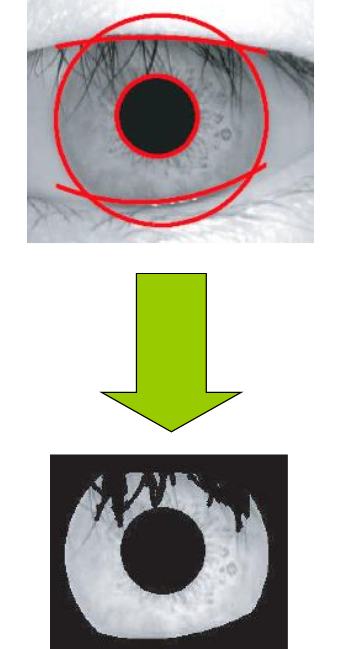
\includegraphics[width=0.3\linewidth]{images/estrazione-ciglia.png}
\end{figure}

\chapter{Algoritmi di matching e prestazioni}

\begin{figure}[ht]
    \centering
    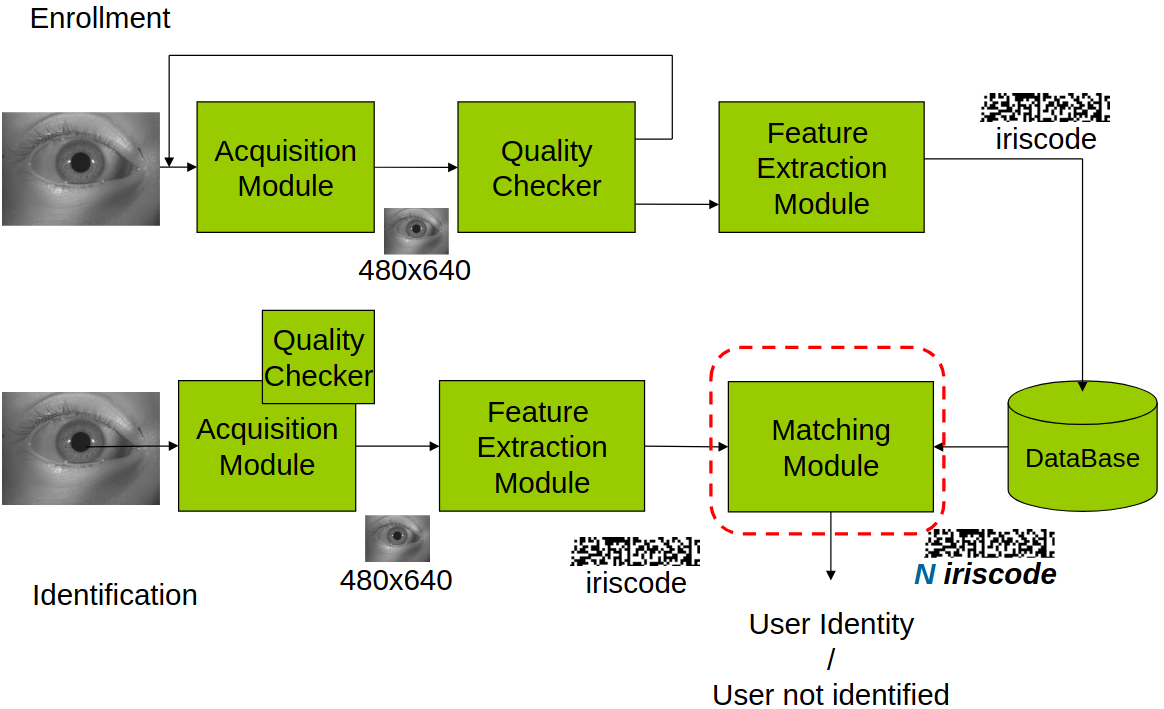
\includegraphics[width=1\linewidth]{images/intro-chap3.png}
\end{figure}

\section{Distribuzione dei bit nell'iriscode}
La probabilità che un bit sia 1 oppure 0 in un iriscode è 
intorno al 50\%, rendendolo un codice a \textbf{massima entropia}.

\noindent Sono presenti tuttavia delle correlazioni fra i bit all'interno 
dell'iriscode:
\begin{itemize}
    \item la struttura è auto-predittiva; alcuni gruppi di bit portano ad incontrare nell'iriscode 
    con maggiore probabilità altri gruppi di bit 
    \item viene limitato il grado di libertà di un iriscode, non è "del tutto casuale"
\end{itemize}

\section{Alcuni fattori che aumentano la variabilità intraclasse}

\begin{figure}[ht]
    \centering
    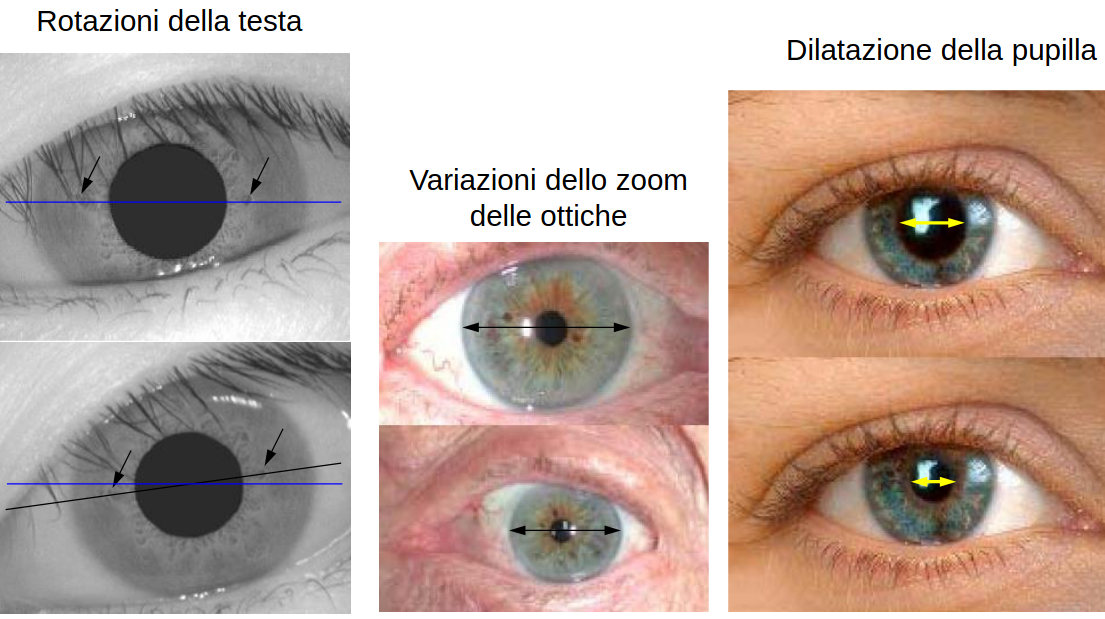
\includegraphics[width=0.9\linewidth]{images/variabilita-intraclasse.png}
\end{figure}

\section{Algoritmi di matching}
La comparazione viene effettuata su iriscode di 256 byte, attraverso 
il calcolo della \textbf{distanza di Hamming}, che conta i bit 
in disaccordo fra le due stringhe.

\noindent In teoria, due iriscode calcolati dall'iride della stessa persona
dovrebbero avere la distanza di Hamming = 0:
\begin{itemize}
    \item in realtà, fra due acquisizioni eseguite perfettamente a pochi 
    istanti una dall'altra si possono osservare delle differenze

    $\rightarrow$ vengono fatte 3 comparazioni e si sceglie quella con valore minimo (della distanza)
    \item nella seconda e terza comparazione, i bit di uno dei due template vengono shiftati rispettivamente a sinistra e poi a destra
\end{itemize}

\section{Maschere}

\subsection{Creazione delle maschere}
Se vi sono delle occlusione dell'iride (palpebre, riflessi, ciglia) occorre 
preparare delle maschere di oscuramento delle zone dove non vi è 
informazione utile.

\begin{figure}[ht]
    \centering
    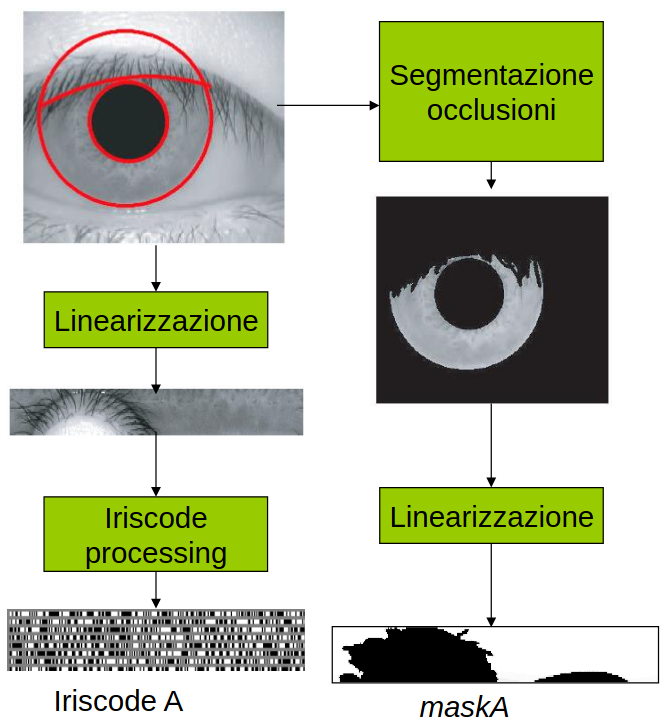
\includegraphics[width=0.5\linewidth]{images/creazione-maschere.png}
\end{figure}

\subsection{Uso delle maschere}

Si va a togliere dalla distanza di Hamming le zone che non 
devono essere cosiderate.

\section{Velocità del matching}
L'esecuzione degli AND e XOR può avvenire a blocchi di bit pari 
alla lunghezza di parola del processore, rendendo il processo 
di matching veloce.

\newpage
\section{Distribuzione del match score}

\begin{figure}[ht]
    \centering
    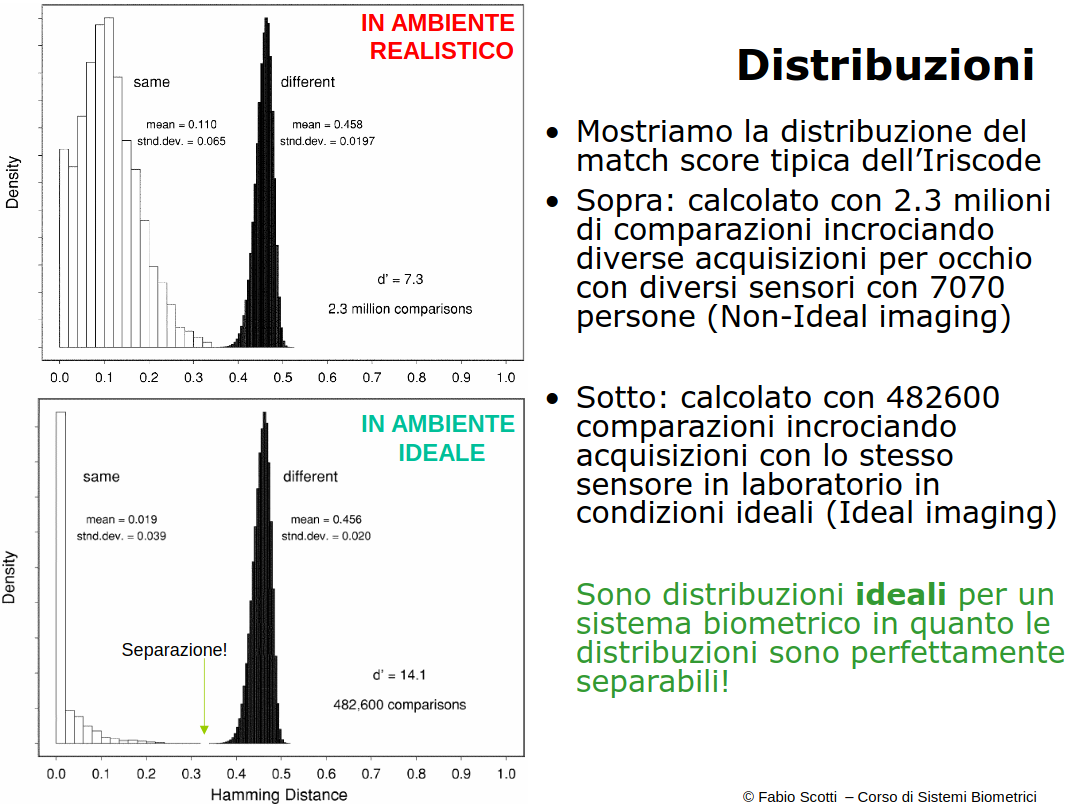
\includegraphics[width=1\linewidth]{images/distr-match-score.png}
\end{figure}

\newpage
\section{Svantaggi della tecnica}
\begin{itemize}
    \item L'utente deve essere collaborarivo e stare esattamente ad una 
    distanza dal sensore o passare da un tornello 
    \item I costi del sensore e del sistema sono alti 
    \item Le immagini possono essere di bassa qualità e provocare errori di \textbf{Failure To Enroll (FTE)}
\end{itemize}

\subsection{FTA e FTE iride}
Non è banale indicare delle cifre esatte per il \textbf{Failure To Acquire (FTA)}
e il \textbf{Failure To Enroll (FTE)} per l'iride, dato che dipende da molti 
fattori, come ad esempio:
\begin{itemize}
    \item qualità dell'immagine 
    \item cooperazione dell'utente e protocollo di acquisizione 
    \item condizioni ambientali 
    \item caratteristiche fisiologiche dell'occhio 
\end{itemize}

\chapter{Spoofing e Anti-Spoofing}

\section{Watch List}
\begin{itemize}
    \item L'iride si presta meglio ad applicazioni con livelli di sicurezza e dimensioni elevate 
    \item Il bassissimo tasso di FMR (\textit{dire che tu sei un altro}) dei sistemi basati sull'iride 
    rende la tecnica \textbf{perfetta per la scansione di enormi DB anche a livello nazionale}
    \item L'iride attualmente è l'unico sistema che offre la scansione realtime di una singola iride con un DB di 
    milioni di iridi
\end{itemize}

\section{Problemi di privacy}
L'exploit di Dougman (riconoscimento con iride di una foto ad alta risoluzione 
nel visibile a 18 anni di distanza) mostra la possibilità del pericolo di 
screening di massa dagli archivi di foto;
i fattori chiave sono:
\begin{itemize}
    \item miglioramente delle tecniche di segmentazione ed estrazione iriscode 
    nel visibile 
    \item sempre maggiore risoluzione nelle foto 
    \item FMR molto bassi 
\end{itemize}

\noindent $\rightarrow$ \textbf{rappresenta un enorme problema di privacy nel futuro}

\section{Frodi attuabili sul sistema}
Esistono molti (non banali) modi di frodare un sistema biometrico:
\begin{itemize}
    \item attaccare i canali di comunicazione del sistema (replay attacks), specialmente 
    il canale di comunicazione dal sensore al sistema 
    \item attaccare dei moduli specifici (sostituire il modulo SW di estrazione di caratteristica o modulo di matching con un Cavallo di Troia)
    \item attaccare il DB con tutti i dati di enrollment 
    \item ingannare il sensore, di solito presentando una iride finta
\end{itemize}

\begin{figure}[ht]
    \centering
    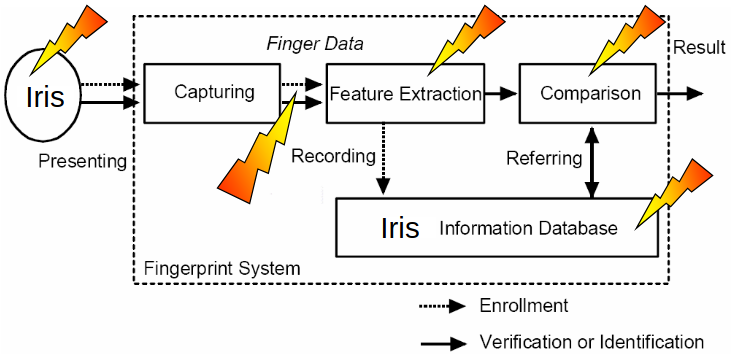
\includegraphics[width=0.8\linewidth]{images/frodi.png}
\end{figure}

\subsection{Attacchi al sensore}
\begin{itemize}
    \item Un attacco piuttosto semplice può consistere nel proporre una fotografia;
    alcuni sistemi che non hanno test di liveness possono essere ingannati
    \item Una iride falsificata mediante una lente a contatto stampata presenta molte 
    delle caratteristiche di liveness, tra cui:
    \begin{itemize}
        \item spostamenti
        \item pupilla di dimensioni variabili 
        \item materiale biologico 
    \end{itemize}
\end{itemize}

\section{Possibili controlli}

\subsection{Tempi di reazione della pupilla}
\begin{itemize}
    \item La pupilla reagisce alle variazioni di luci ambientali, un occhio finto no 
    \item La velocità di contrazione e dilatazione sono diverse ed hanno un andamento prefissato (l'occhio 
    è in grado di proteggersi chiudendosi più velocemente, rispetto a quanto impiega per aprirsi)
\end{itemize}

\subsection{Spettrometria e termografia dell'occhio}
\begin{itemize}
    \item Usando illuminatori a frequenze ottiche diverse è possibile avere in tempo reale una spettrografia dell'iride 
    \item Attraverso altri strumenti che analizzano lo spettrogramma si stima il materiale con cui è composta 
    
    $\rightarrow$ permette di controllare se è di tipo organico oppure è finta
    \item Anche con una immagine termografica si può controllare se abbiamo di fronte 
    un tessuto a temperatura corretta
\end{itemize}

\section{Altre contromisure: permutazioni}
\textit{"se viene rubato il mio iriscode, non posso cambiare il mio occhio!"}

\noindent Si usano $256!$ possibili schemi di permutazione (sulle iridi da
comparare) facendo diventare il vecchio iriscode inservibile.

\begin{figure}[ht]
    \centering
    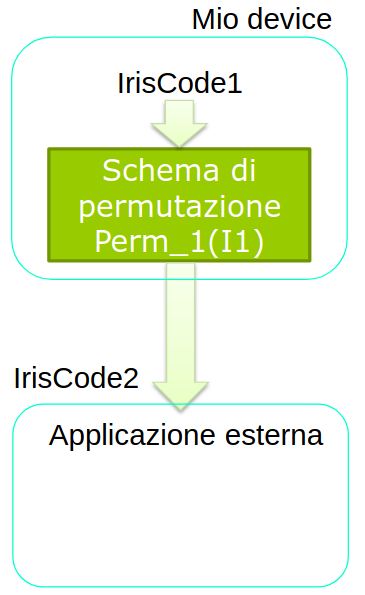
\includegraphics[width=0.3\linewidth]{images/permutazioni.png}
\end{figure}

\noindent Lo XOR non risente delle permutazioni:
\begin{itemize}
    \item $XOR(A,B) = XOR( Perm(A), Perm(B))$
\end{itemize}

\section{Generazione sintetica di iridi}
\begin{itemize}
    \item Una tecnica usa algoritmi iterativi per la generazione sintetica di pattern:
    \begin{itemize}
        \item si parte da piccole porzioni di immagine reale (primitive)
        \item si crea una matrice casuale 
        \item le primitive vengono mischiate casualmente in modo iterativo
    \end{itemize}
    \item Un'altra tipologia sono le tecniche a multistrato che imitano la vera fisologia dell'iride:
    \begin{itemize}
        \item si prepara un modelo 3D dell'iride 
        \item si preparano gli strati con delle texture orientate in modo pseudo-casuale 
        \item si sovrappongono gli strati tenendo conto delle trasparenze 
        \item si adatta l'immagine degli strati al modello 3D, calcolando anche le luci ed ombre
    \end{itemize}
\end{itemize}

\noindent Entrambi gli approcci sono oggi possibili anche con reti neurali.







\end{document}